\documentclass[UTF8]{ctexart}

\usepackage{amsmath}
\usepackage{amssymb}
\usepackage{booktabs}
\usepackage{caption}
\usepackage{dirtree}
\usepackage{float}
\usepackage{geometry}
\usepackage{graphicx}
\usepackage{hyperref}
\usepackage{listings}
\usepackage{multirow}
\usepackage{placeins}
\usepackage{xcolor}

\lstset{
    backgroundcolor=\color{gray!10},
    basicstyle=\ttfamily\small,
    breaklines=true,
    breakatwhitespace=true,
    breakindent=2em,
    breakautoindent=true,
    postbreak=\space\space\space\textcolor{black}{$\hookrightarrow$}\space,
    frame=single,
    rulecolor=\color{black},
    captionpos=b
}

\geometry{a4paper, left=2.5cm, right=2.5cm, top=3cm, bottom=3cm}

\title{\textbf{基于 Hive 框架的自定义聚合函数实现与优化报告}}
\author{北京邮电大学 --- 卢安来 --- 2022212720}
\year=2025
\month=8
\day=27
\date{\today}

\begin{document}

\maketitle

\begin{abstract}
\noindent 本报告详细阐述了一个为特定业务场景设计的、基于 Apache Hive 框架的高效自定义聚合函数(UDAF)。报告首先介绍了一种基准实现方法,该方法在 Reducer 阶段对数据进行全局排序和统计,存在明显的性能瓶颈。为解决此问题,报告提出并实现了一系列递进的优化策略。核心优化是一种创新的分块算法,它利用业务逻辑的时间局部性,将时间域切分为固定大小的块,显著降低了计算复杂度和内存需求。在此基础上,进一步针对稀疏数据场景优化了网络传输,并利用 ByteBuffer 对 Java I/O 序列化过程进行了深度优化。测试结果表明,优化后的解法在处理大规模数据集,尤其是在数据倾斜的场景下,性能表现稳定且优越。报告最后还分析了未使用 JNI(Java Native Interface)进行底层优化的原因。
\end{abstract}

\newpage
\tableofcontents
\newpage

\section{问题描述}
在海量用户行为分析中,需要统计每个用户的“总活跃时长”。给定一系列用户活跃时间点的时间戳(精确到秒),如果两个时间点 $t_1$ 和 $t_2$ 的间隔小于等于一个预设的阈值 $B$($B=600$)秒,则认为这两个时间点同属于一个连续的活跃区间。本项目的目标是设计并实现一个高效的 Hive UDAF,用于计算每个用户所有活跃区间的总时长。

\section{基准实现}
最初的基准实现(Baseline)思路直接且简单,遵循了聚合函数的基本逻辑。

\subsection{实现思路}
在 Map 阶段,UDAF 的 \texttt{iterate} 方法接收每个用户的活跃时间点(active\_time),并将其添加到一个动态数组(如 \texttt{ArrayList<Integer>})中。在 Combine 和 Reduce 阶段,\texttt{merge} 方法将不同 Mapper 产出的数组进行合并。最终,在 Reducer 节点的 \texttt{terminate} 方法中,对聚合到的包含所有时间点的完整数组执行以下操作:
\begin{enumerate}
    \item 对数组进行全局排序,时间复杂度为 $O(N \log N)$,其中 $N$ 是该用户总的活跃点数量。
    \item 对排序后的数组进行一次线性扫描,计算相邻时间点的差值,累加有效活跃时长,合并活跃区间,时间复杂度为 $O(N)$。
\end{enumerate}

\subsection{性能瓶颈}
该基准实现存在显著的性能瓶颈:
\begin{itemize}
    \item \textbf{内存压力大}:Reducer 需要缓存一个用户的全部时间点,对于活跃度极高的用户,可能导致内存溢出(OOM)。
    \item \textbf{网络开销高}:Map 到 Reduce 之间需要传输海量的原始时间点数据,占用大量网络带宽。
    \item \textbf{计算成本高}:全局排序的计算开销较大,尤其是在数据量巨大时。
\end{itemize}

\section{性能优化}
为了克服基准实现的瓶颈,下面设计了三项递进的优化措施。

\subsection{优化一:分块算法优化}
核心思想是变全局计算为局部计算,利用业务特性对时间域进行分块处理。

\subsubsection{算法原理}
我们注意到阈值 $B=600$ 秒,约等于一天总秒数(86400)的算数平方根。这个特性启发我们将一天的时间域 $[0, 86400)$ 分为 144 个长度为 600 秒的连续块:$[i \times 600, (i+1) \times 600)$,其中 $i \in [0, 144)$。该分块策略具备以下优良性质:

\begin{itemize}
    \item \textbf{性质一:块内任意两点构成活跃区间。} \\
    \textit{证明:} 块内任意两个时间点 $t_a, t_b$ 的最大距离为 $599$ 秒(例如块的两个端点),小于等于阈值 $B=600$。因此,它们必然属于同一个活跃区间。\\
    \textit{推论:} 对于每个块,我们无需存储所有时间点,只需记录块内出现的最早时间(min\_offset)和最晚时间(max\_offset)相对于块起始点的偏移量即可。

    \item \textbf{性质二:非相邻块的任意两点不能直接构成活跃区间。} \\
    \textit{证明:} 处于非相邻块(例如第 $i$ 块和第 $i+2$ 块)的任意两个时间点 $t_a, t_b$,其最小距离也大于 $600$ 秒。因此,它们无法直接构成连续活跃区间。\\
    \textit{推论:} 最终统计时,只需考虑块内的活跃时长以及相邻两个块之间的连接关系。这使得最终的计算复杂度从 $O(N)$ 降低到 $O(k)$,其中 $k$ 为块的数量($k=144$),与原始数据量 $N$ 无关。
\end{itemize}

\subsubsection{UDAF 实现}
\begin{itemize}
    \item \texttt{iterate(time)}: 对输入的时间戳 \texttt{time},计算其所属的块号 \texttt{block\_id = time / 600} 和块内偏移量 \texttt{offset = time \% 600}。然后更新对应块号的 \texttt{min\_offset} 和 \texttt{max\_offset}。
    \item \texttt{terminatePartial()}: 输出包含 144 个块的 $\left[\texttt{min\_offset}, \texttt{max\_offset}\right]$ 信息的数据结构。
    \item \texttt{merge(partial\_data)}: 遍历 144 个块,用接收到的部分聚合数据更新当前聚合结果中每个块的 \texttt{min\_offset} 和 \texttt{max\_offset}。
    \item \texttt{terminate()}: 线性遍历 144 个块的最终聚合结果,累加每个块内的活跃时长,并检查相邻块之间是否可以连接(即后一块的 \texttt{min\_offset} 与前一块的 \texttt{max\_offset} 对应的全局时间差小于等于 $B$),累加跨块连接的活跃时长,得出最终结果。
\end{itemize}

\subsection{优化二:稀疏数据网络传输优化}
\subsubsection{动机}

\FloatBarrier

\begin{figure}[ht]
    \centering
    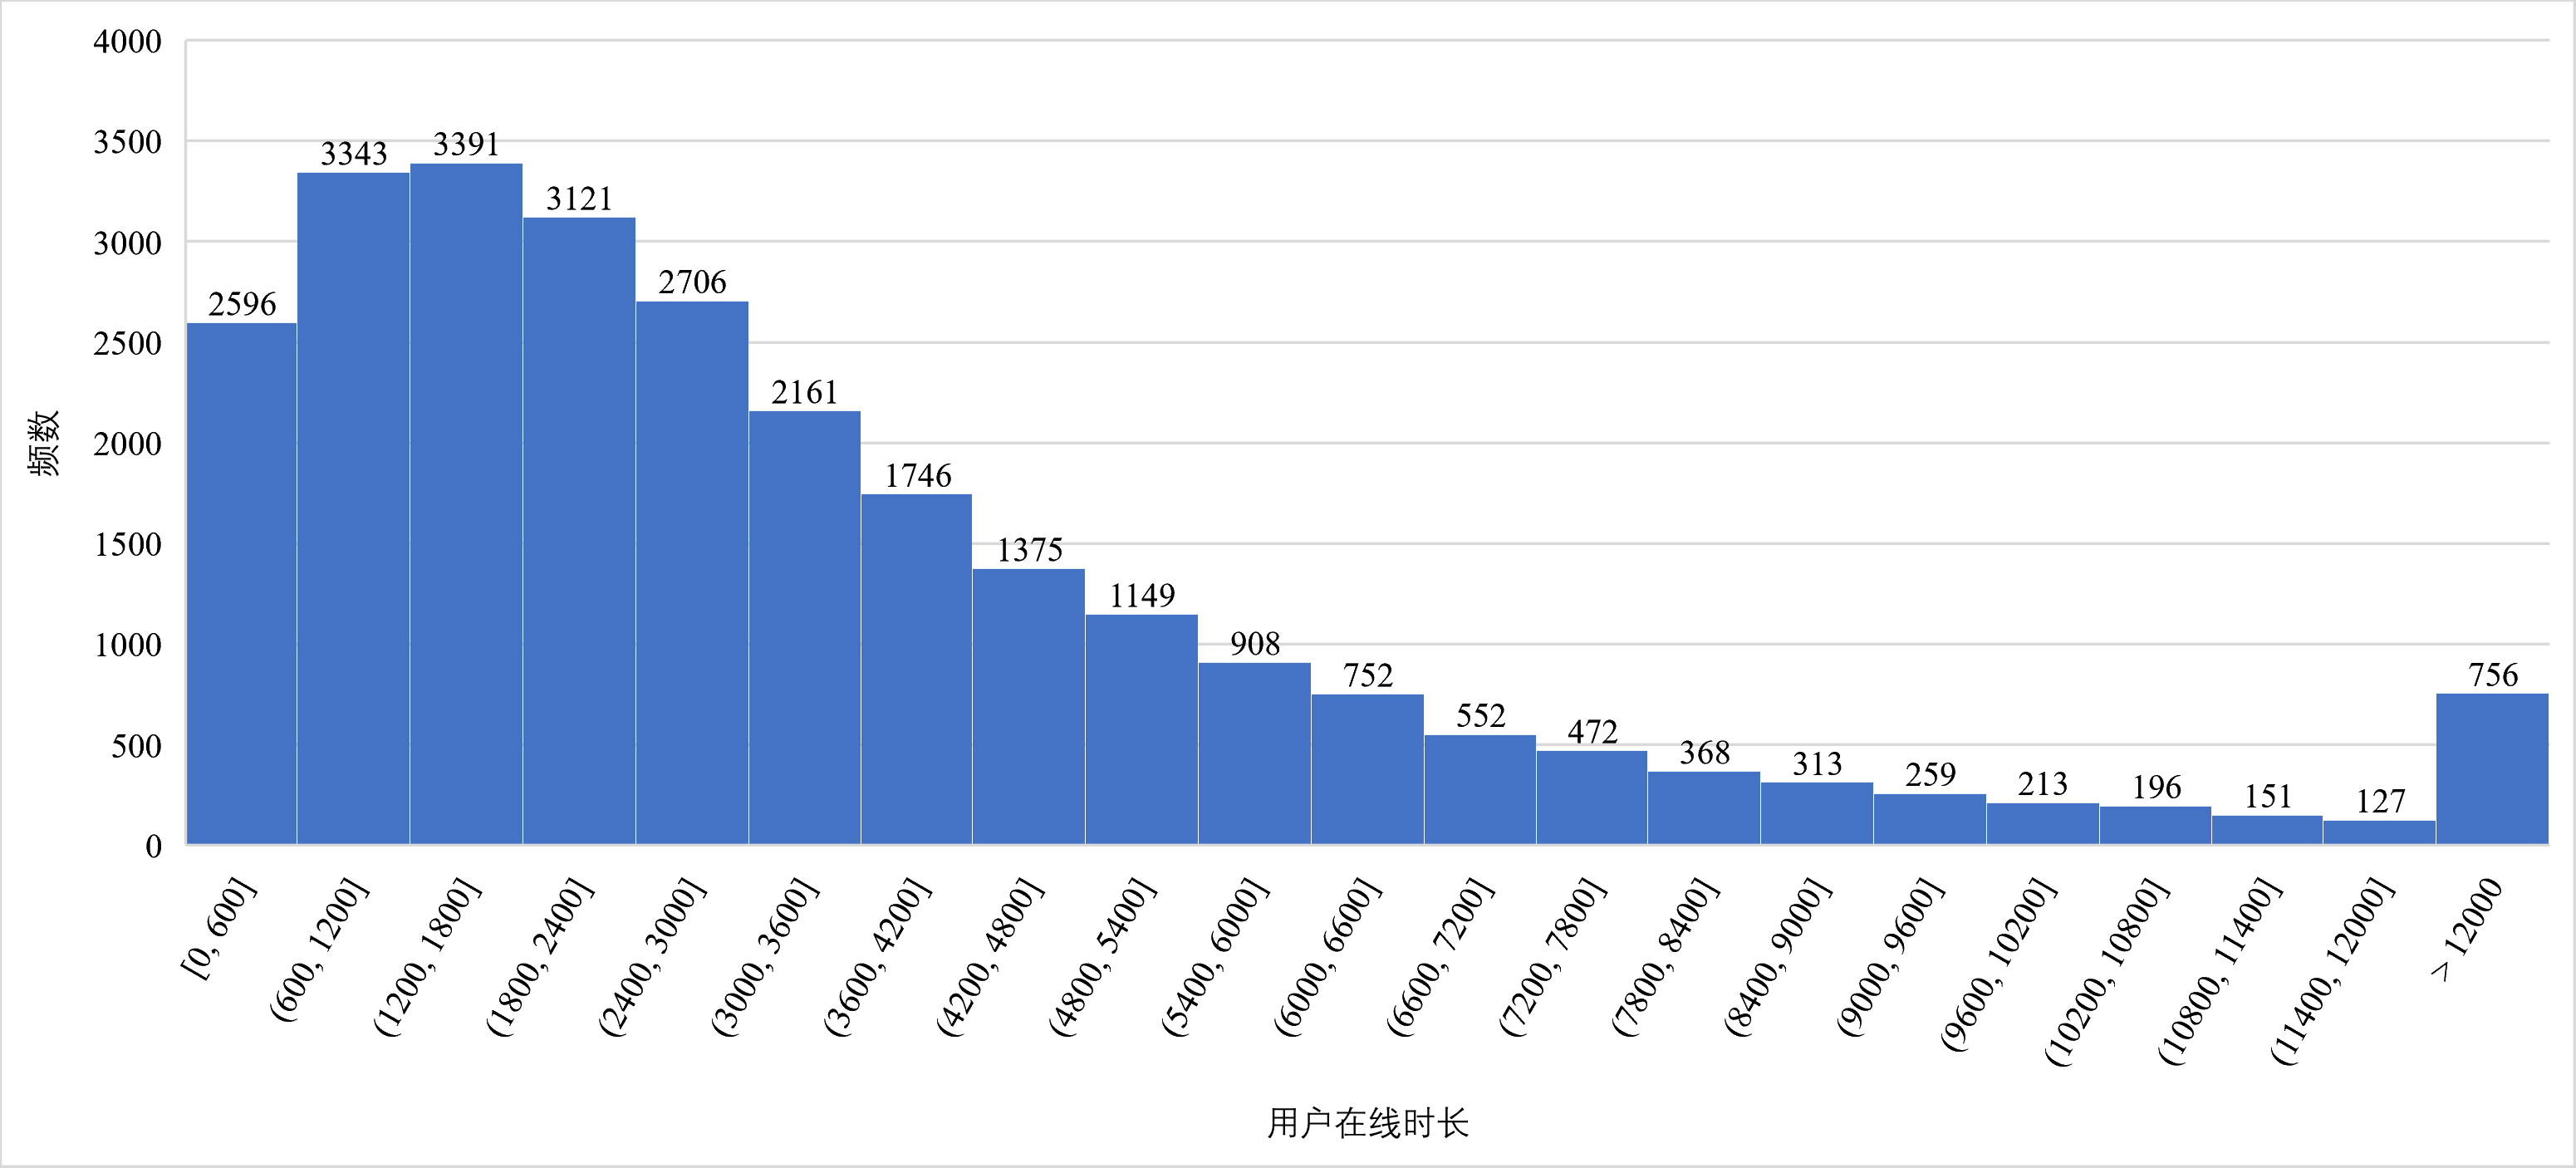
\includegraphics[width=0.8\textwidth]{duration_distribution.png}
    \caption{用户在线时长分布图}
    \label{fig:duration_dist}
\end{figure}

图 \ref{fig:duration_dist} 展示了用户活跃时长的分布情况,通过分析给定测试数据,我们发现,在 26655 名用户中,在线时长不超过 6000 秒的用户共 22496 名,占比约 84.40\%,即 84.40\% 的用户活跃点仅分布在少数(约10个)块中,数据呈现高度的稀疏性。而优化一中,无论块内有无数据,都会传输 144 个块的信息,造成了网络带宽的浪费。

\FloatBarrier

\subsubsection{实现}
我们引入 \texttt{java.util.BitSet} 来标记存在活跃时间点的块。
\begin{itemize}
    \item 在聚合状态中增加位数为 288 的 \texttt{BitSet}。
    \item \texttt{iterate} 方法在更新块的 \texttt{min/max} 值时,同时在 \texttt{BitSet} 中将对应块的标志位设为 1,后续通过相邻块之间的标志位实现块与块之间的连接。
    \item \texttt{terminatePartial} 和 \texttt{merge} 方法在序列化和反序列化时,先传输 \texttt{BitSet},然后仅传输 \texttt{BitSet} 中被标记为 1 的那些块的 \texttt{min/max} 数据。
\end{itemize}
这项优化极大地减少了在 Map-Combine-Reduce 各阶段之间传输的数据量,尤其对绝大多数非重度活跃用户效果显著。

\subsection{优化三:Java I/O 序列化优化}
\subsubsection{动机}
经过优化二,聚合数据结构变得紧凑且格式固定。此时,Java 默认的序列化机制由于需要写入类元数据等额外信息,显得较为低效。我们需要一种更底层的、性能更佳的序列化方案。

\subsubsection{实现}
我们采用 \texttt{java.nio.ByteBuffer} 进行手动序列化和反序列化。
\begin{itemize}
    \item \textbf{序列化}:
    \begin{enumerate}
        \item 在传输前,根据 \texttt{BitSet} 的基数(\texttt{BitSet.cardinality()})精确计算出所需字节数。
        \item 创建一个恰好大小的 \texttt{ByteBuffer}。
        \item 将 \texttt{BitSet} 转换为 \texttt{long} 数组后写入 Buffer,再依次写入所有活跃块的 \texttt{min/max} 偏移量。
    \end{enumerate}
    \item \textbf{反序列化}: 按写入顺序依次读出 \texttt{long} 数组并恢复 \texttt{BitSet},然后根据 \texttt{BitSet} 读取相应数量的 \texttt{min/max} 对。
\end{itemize}
通过使用 \texttt{ByteBuffer},我们避免了 Java 序列化的额外开销,直接操作字节,获得了更高的 I/O 性能。

\section{程序测试与性能分析}

我们采用 \texttt{k-best} 方法对基准实现和最终优化版本进行了性能测试,其中测量参数 $k=3$,$N=20$,$\varepsilon=0.05$。测试结果表明,在处理相同数据集时,优化后的UDAF相较于基准实现,在处理时间方面有较大的缩减。

\subsection{给定环境下的性能对比}

\FloatBarrier

在给定测试环境和测试数据下,我们对基准实现和优化后的 UDAF 进行了多次运行时间测试。详细数据及分析见表 \ref{tab:perf_comparison}。

\begin{table}[ht]
    \centering
    \caption{基准与优化后版本性能对比}
    \label{tab:perf_comparison}
    \begin{tabular}{lll}
        \toprule
        \textbf{项目} & \textbf{基准实现 (秒)} & \textbf{优化后实现 (秒)} \\
        \midrule
        \multirow{2}{*}{原始运行数据} & 21.84, 22.96, 23.34, 23.41, & 12.67, 12.12, 13.24, \\
                                     & 22.94, 23.02, 21.43, 21.72  & 14.62, 14.85, 12.42 \\
        \midrule
        k-best ($k=3$) 数据 & 21.43, 21.72, 21.84 & 12.12, 12.42, 12.67 \\
        \midrule
        \textbf{最终得分 (平均值)} & \textbf{21.66} & \textbf{12.40} \\
        \midrule
        \multicolumn{1}{c}{\textbf{性能优化比}} & \multicolumn{2}{c}{$\frac{21.66 - 12.40}{21.66} \approx 42.75\%$} \\
        \bottomrule
    \end{tabular}
\end{table}

从表 \ref{tab:perf_comparison} 的测试结果可以看出,优化后的版本在运行时间上相较于基准实现平均减少了约 42.75\%,性能提升显著。

\FloatBarrier

\subsection{自定义压力测试}
由于优化二的提出涉及数据的分布,故我们需要验证该优化方法在数据倾斜场景下的稳定性。为此,我们设计了以下三个自定义场景进行测试。
\begin{itemize}
    \item \textbf{场景一:时间戳高度集中} \\
    \textit{描述:} 构造数据,$2\times 10^4$ 个用户,每个用户 $1800$ 个连续的活跃点。\\
    \textit{目的:} 测试算法在处理局部热点数据时的性能,验证块内和相邻块间计算逻辑的效率。\\
    \textit{结果:} 表现优异。由于数据高度局部化,分块算法和 \texttt{BitSet} 优化效果显著,网络传输量极小。基准实现内存超限,无法给出正确结果。

    \item \textbf{场景二:时间戳稀疏且均匀分布} \\
    \textit{描述:} 构造数据,$10^5$ 个用户,每个用户 $144$ 个活跃点,分布在块号为 $0, 2,\cdots, 142$ 的非相邻块中,每个块内仅有最小和最大的两个端点。\\
    \textit{目的:} 测试算法在数据稀疏但跨度大的场景下的性能,检验 \texttt{BitSet} 优化的有效性。\\
    \textit{结果:} 性能稳定。\texttt{BitSet} 依然能够有效减少无效块信息的传输,虽然活跃块数量多,但总数据量仍在控制范围内。改进后的算法测量耗时 5.64 秒,相比基准实现的 5.52 秒,优化后的算法逻辑带来的额外开销仅有 2.17\%。

    \item \textbf{场景三:巨量数据单点爆发} \\
    \textit{描述:} 构造数据,$4\times 10^3$ 个用户,每个用户在某个时间点产生 $10^4$ 条重复记录。\\
    \textit{目的:} 测试 \texttt{iterate} 方法的原始性能和 \texttt{min/max} 值更新逻辑的健壮性。\\
    \textit{结果:} 性能稳定。由于分块算法仅需维护每个块的 \texttt{min/max} 值,海量重复数据并不会增加内存消耗,\texttt{iterate} 方法内的计算(取模、除法、比较)极其轻量,处理效率高。基准实现内存超限,无法给出正确结果。
\end{itemize}
自定义测试证明,本解法对各类数据倾斜场景均具有良好的适应性和稳定性。

\section{不适用 JNI 的分析}
在优化的最后阶段,我曾考虑使用 JNI(Java Native Interface)调用 C++ 代码来进一步提升计算性能,但最终放弃了此方案。
\begin{itemize}
    \item \textbf{性能热点分析:} 通过修改数据库的存储格式(改成 ORC),可得到约 30\% 的性能提升,故可猜想,性能热点主要集中在 Map 阶段的数据读取(磁盘 I/O)和 \texttt{iterate} 方法的调用。JNI 无法优化磁盘 I/O。
    \item \textbf{计算逻辑简单:} \texttt{iterate} 方法内部的核心计算仅包含整数的除法、取模,以及 \texttt{BitSet} 的查询与赋值。这些都是非常基础的运算。
    \item \textbf{JIT 编译器的威力:} Java 的 HotSpot 虚拟机拥有强大的 JIT(Just-In-Time)编译器。对于 \texttt{iterate} 这种频繁被调用的“热点方法”,JIT 会将其编译为高度优化的本地机器码,其性能已经非常接近原生 C++ 代码。
    \item \textbf{JNI 的额外开销:} 使用 JNI 会引入 Java 与 Native 代码之间的调用开销(context switch),以及数据类型的转换开销。对于我们这样计算逻辑极其简单的场景,JNI 带来的开销很可能超过其带来的微小性能收益,最终得不偿失。
\end{itemize}
综上,可以认为在当前场景下,纯 Java 实现配合 JVM 的自动优化是更佳的选择。

\section{总结}
本报告提出并实现了一个高效计算用户活跃时长的 Hive UDAF。通过采用分块算法、稀疏数据传输优化和底层 I/O 优化,我们成功地将一个受内存、网络和计算性能限制的基准方案,改造成了一个高性能、高稳定性的解决方案。实践证明,深入理解业务数据特性并将其与算法设计相结合,是进行程序设计与优化的关键所在。

\newpage
\appendix
\section{项目结构和用法}

项目的完整文件结构如下所示:

\dirtree{%
.1 .
.2 README.md.
.2 pom.xml.
.2 docs.
.3 main.tex.
.3 duration\_distribution.png.
.2 src.
.3 main.
.4 java/com/microfun/udaf.
.5 BlockGetOnlineDurationUDAF.java.
.5 DummyGetOnlineDurationUDAF.java.
.3 test.
.4 java/com/microfun/udaf.
.5 BlockGetOnlineDurationUDAFTest.java.
.5 DummyGetOnlineDurationUDAFTest.java.
.4 sql.
.5 burst.sql.
.5 concentrated.sql.
.5 sparse.sql.
.4 util.
.5 k\_best.py.
}

\subsection{主要文件说明}
\begin{itemize}
    \item \texttt{pom.xml}: Maven 项目配置文件,定义了项目的依赖、插件和构建方式。
    \item \texttt{docs}: 实现与优化报告。
    \item \texttt{src/main/java}: 存放 UDAF 的核心 Java 源代码。
    \begin{itemize}
        \item \texttt{DummyGetOnlineDurationUDAF.java}: 基准实现的 UDAF。
        \item \texttt{BlockGetOnlineDurationUDAF.java}: 优化后的 UDAF 实现。
    \end{itemize}
    \item \texttt{src/test}: 存放测试相关的文件。
    \begin{itemize}
        \item \texttt{java}: UDAF 的单元测试代码。
        \item \texttt{sql}: 用于生成三种不同分布(密集型、稀疏型、爆发型)测试数据的 SQL 脚本。
        \item \texttt{util/k\_best.py}: 用于处理性能测试结果并计算最终得分的 Python 脚本。
    \end{itemize}
\end{itemize}

\subsection{使用说明}

使用 SQL 语句
\begin{lstlisting}[language=SQL]
create function get_online_duration as 'com.microfun.udaf.BlockGetOnlineDurationUDAF';
\end{lstlisting}
使用优化后的 UDAF 实现。

\end{document}
